\documentclass[12pt, spanish, pdftex]{UC3M_document}

%%%%% Preamble %%%%%
\author{Jorge Rodríguez Fraile}
\authorstwotrue
\authorsuptothree{Jorge Rodríguez Fraile}{100405951}{Grupo 83}{}{}{}{}{}{}


%%%%% Basic data about the document (Degree, subject, title, campus, page number custom text) %%%%%
\documentdata{Grado en Ingeniería Informática}{Algoritmos Genéticos y Evolutivos}{Práctica 2 \\ Calibración de motores automática mediante Estrategias Evolutivas}{Leganés}{}

%%%%% Page style %%%%%
\header
\footer
\pagestyle{fancy}

\begin{document}
%%%%% Page title %%%%%
\begin{titlepage}
	\centeredtitle{img/LogoUC3M.png}{\studyname}{Curso 2021-2022}{\subjectname}{\documenttitle}
	
	\begin{table}[b]
		\centering
		\begin{tabular}{ cccc }
			\large Jorge Rodríguez Fraile & \large 100405951 & \large Grupo 83 & \href{mailto:100405951@alumnos.uc3m.es}{\large 100405951@alumnos.uc3m.es} \\
			                              &                  &                 &                                                                           \\
			                              &                  &                 &                                                                           \\
		\end{tabular}
	\end{table}
	
\end{titlepage}

\newpage

%%%%% Index %%%%%
\begin{spacing}{0.5}
	% \shipout\null                   % Blank page before index (after title page)
	\hypersetup{linkcolor=black}    % References/links on the index will remain black color
	\tableofcontents\newpage        % Index of the document
	\listoffigures\newpage          % Index of pictures
	\listoftables\newpage           % Index of tables
\end{spacing}


%%%%% DOCUMENT CONTENT %%%%%
\section{Introducción}
Este proyecto trata sobre encontrar una aproximación mediante estrategias evolutivas al problema de calibrar motores de un brazo robótico utilizando solo un láser, una cámara y un objeto de referencia. El robot deberá ser preciso en sus movimientos, dado que será utilizado para realizar soldaduras de alta precisión.

Para comenzar se trabajará sobre un brazo compuesto solo por 4 motores para podernos acercar al problema de una manera más gradual, en cuanto se haya comprobado que es factible esta simplificación del problema se pasara a un caso más realista con un brazo de 10 motores.

\section{Codificación y Función de fitness}
Al emplear estrategias evolutivas la codificación de los individuos de este problema consistirá en un vector de codificación compuesto por 4 o 10 números reales (según el número de motores) y un vector de varianzas de la misma longitud que el de codificación.

Los valores del vector de codificación estarán centrados en 0 representando que no se ha realizado ningún giro y podrán rotar tanto como quieran en sentido positivo como negativo, aunque llegado un punto girar mucho en un sentido equivale a movimientos más cortos. Lo ideal es que los valores se muevan entre -180 y 180 grados representando un giro completo de 360 grados, aunque no se restringirán los valores que puede tomar.
\begin{figure}[H]
	\ffigbox[\FBwidth]
	{\caption{Diagrama brazo robótico}}
	{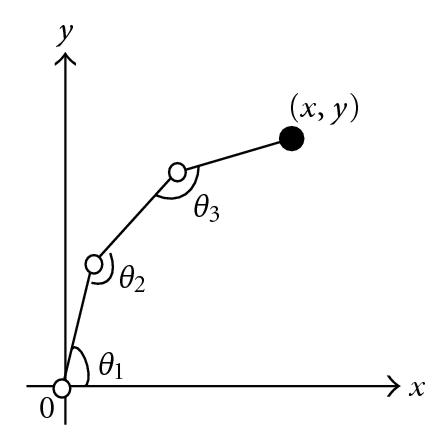
\includegraphics[scale=1.5]{./img/arm_angles.jpg}}
\end{figure}

En cuanto a la función de fitness que se empleará para saber si una solución es buena o no, esta tendrá en cuenta el error que comente el soldador en un simulador, según como de dispersos y desviados sean con respecto al centro dará un valor mayor cuanto peor lo haga y menor cuanto más preciso sea. Por lo que el objetivo del problema es minimizar la función de fitness.

Para conocer el error para cada una se las soluciones se hará una llamada get a un servicio que se encuentra en un servidor de la universidad, \href{http://memento.evannai.inf.uc3m.es/age/robot4?}{http://memento.evannai.inf.uc3m.es/age/robot4?}, seguido de cX=GradosDeX para cada uno de los 4 motores y separados por un $\&$, en el caso de los 10 motores será igual, aunque con otro servicio \href{http://memento.evannai.inf.uc3m.es/age/robot10?}{http://memento.evannai.inf.uc3m.es/age/robot10?} y 10 valores de grados.

\section{Programación Estrategia Evolutiva (1+1)}
Para este proyecto entre las posibles implementaciones de las estrategias evolutivas se ha elegido la (1+1)-EE y a continuación se describirán las características de esta. 

El programa se ha desarrollado en el lenguaje Python, el procesamiento principal del programado se encuentra en la función \textit{EE1plus1(c, cycles, test\_iteration)}, donde recibirá como parámetros el valor por el que se multiplicaran las varianzas, el número de generaciones máximas del programa y la iteración en la que se encuentra el programa (se incluye para realizar las pruebas de ejecutar múltiples veces).

El proceso que sigue esta función es el siguiente:
\begin{enumerate}
	\item Generar el individuo inicial.
	\item Evaluar el individuo generado de la población inicial.
	\item Repetir hasta cumplir el criterio de convergencia:
	      \begin{enumerate}
		      \item Generar una nueva solución a partir del único individuo de la población, mutando el vector de codificación del descendiente.
		      \item Evaluar el individuo generado.
		      \item Eliminar el individuo cuyo valor de adecuación sea mayor, tratamos de minimizar el fitness.
		      \item Si el individuo que queda es el nuevo, se aumenta la frecuencia de éxitos y si no se disminuye.
		      \item Mutar el vector de varianzas del individuo elegido de acuerdo con la regla 1/5.
	      \end{enumerate}
\end{enumerate}

Además de lo relacionado con la generación de individuos, también se ha incluido código que nos permita almacenar la salida de los modelos para poderlos evaluar.

\subsection{Operadores genéticos}
\subsubsection{Población inicial}
El individuo inicial es generado aleatoriamente, su vector de codificación siguiendo una gaussiana centrada en 0 y con desviación 100, de esta manera los valores serán tanto positivos como negativos y mayoritariamente centrado en 0, por otro lado el vector de varianzas se genera mediante valores reales positivos entre 5 y 20, aunque se realizarán pruebas con valores mayores.

Este proceso es realizado por la función \textit{initial\_individual()}, devolviendo un individuo en forma de matriz NumeroDeMotores x 2.  

\subsubsection{Mutación}
Para los algoritmos evolutivos este operador se realiza en dos partes una para el vector de codificación y otra para el de varianzas.

Para el vector de codificación, el nuevo individuo tendrá como valores los del progenitor más un valor de la normal según la varianza de ese valor para el padre, es decir $x_s=x_p+N_0(\sigma_p)$, esta operación se repite para todos los valores del vector.

En cuanto al vector de varianzas, se realizará sobre el individuo seleccionado para la siguiente generación, y consiste en modificar sus varianzas en función de la regla 1/5, que se guia por el porcentaje de mejoras de las últimas generaciones. Esta regla se aplicará teniendo en cuenta las 10 últimas generaciones, las variaciones vendrán dadas por:
\begin{itemize}
	\item Si el número de mejoras es superior al 20 \%, se aumenta la varianza $\frac \sigma c$.
	\item Si el número de mejoras es inferior al 20 \%, se reduce la varianza $\sigma \cdot c$.
	\item Si el número de mejoras es igual al 20 \%, se mantiene $\sigma$.
\end{itemize}

Lo que dice la regla es que si mejora con frecuencia es que todavía estamos lejos de la solución óptima y si no mejoramos es que estamos cerca y nos moveremos poco a poco.

Esta funcionalidad se encuentra en la función \textit{mutate\_codification(individual)} para el vector de codificación, aplica la operación para codificación y devuelve al sucesor, y en \textit{individual\_next\_generation(individual, son, improvements\_counter, iteration, c)} para el vector de codificación, se encuentran separadas porque hasta que no se conoce el individuo de la siguiente generación no se muta.

\subsubsection{Inserción y Remplazo}
Al tratarse del tipo (1+1) la población está formada por un solo individuo y también habrá un solo individuo, por lo que entre el individuo de la población y el nuevo se elegirá el mejor, en este caso el de menor fitness.

Cuando se elija al descendiente se considera una mejora y se tendrá en cuanta en la frecuencia de mejoras, si no se considera que no ha mejorado. Tras elegir el individuo que formará la población se mutará su vector de varianzas como se ha elegido antes.

La función que recoge la inserción y remplazo, además de la mutación de las varianzas es la que se mencionó antes, \textit{individual\_next\_generation(individual, son, improvements\_counter, iteration, c)}, que evalúa ambos individuos, elige el mejor, actualiza el contador de mejoras y aplica la mutación en función del parámetro c que se le pasa. La función devuelve el individuo elegido, su fitness y el contador de mejoras actualizado. 

\subsection{Aproximación 4 motores}
Comenzaremos realizando pruebas en la versión simplificada del problema, en el que solo se consideraran 4 motores para el brazo soldador. 

Estos primeros modelos que se generaran consistirán en la variación del valor c, el que determina cuanto cambiara la varianza de los individuos. Es conocido que el valor debe ser inferior a 1 y que el recomendable es 0,82, pero en busca de mejores resultados se ha probado además con 0,98, 0, 92, 0,72 y 0,62. No se han variado más estos valores, porque la selección de valores más bajos provocaría que los valores de varianza se movieran muy rápido.

Todos los modelos se han ejecutado durante 5000 generaciones, que son 10000 evaluaciones, y se han realizado 10 ejecuciones para cada modelo para evitar el sesgo de la aleatoriedad a la hora de generar los valores aleatorio.

Los modelos han sido nombrados siguiendo el siguiente patrón evolution\_strategy\_XX\_YY\_A-B\_C:
\begin{itemize}
	\item \textbf{XX:} Indica el número de motores que se consideran y para los que se ajustaran los ángulos.
	\item \textbf{YY:} Indica el valor de c, el cual determina como se modificarán las varianzas.
	\item \textbf{A-B:} Indica el rango de valores entre los que se generan aleatoriamente las varianzas.
	\item \textbf{C:} Indica el número de generaciones que tiene en cuanta para medir la frecuencia de mejora.
\end{itemize}

En la siguiente gráfica se pueden ver los resultados de fitness obtenidos en las 10 ejecuciones para los 5 modelos, junto a la media de cada modelo que es la que utilizaremos para comparar.
\begin{figure}[H]
	\ffigbox[\FBwidth]
	{\caption{Valores de Fitness: 4\_5-20\_10}}
	{\includegraphics[scale=.6]{./img/Fitness\_4\_5-20\_10.png}}
\end{figure}
\begin{table}[H]
	\centering
	\resizebox{\textwidth}{!}{%
		\begin{tabular}{|c|c|c|c|c|c|c|c|c|c|c|c|}
			\hline
			\rowcolor[HTML]{BFBFBF}
			\textbf{Modelo}                                    & \textbf{1}  & \textbf{2}  & \textbf{3}  & \textbf{4}  & \textbf{5}  & \textbf{6}           & \textbf{7}  & \textbf{8}  & \textbf{9}  & \textbf{10} & \textbf{Media}       \\ \hline
			\cellcolor[HTML]{BFBFBF}\textbf{4\_0,98\_5-20\_10} & 399,8967664 & 21,88903367 & 20,89403404 & 1,989918114 & 2,984877171 & \textbf{0,994959057} & 243,1577278 & 13,92939149 & 49,74695184 & 5,969749305 & \textbf{76,14534088} \\ \hline
			\cellcolor[HTML]{BFBFBF}\textbf{4\_0,92\_5-20\_10} & 115,4108682 & 86,56039686 & 587,9440061 & 654,4753316 & 51,73723573 & 25,86868199          & 35,81824234 & 125,3603064 & 2081,267141 & 4,974790248 & 376,9417             \\ \hline
			\cellcolor[HTML]{BFBFBF}\textbf{4\_0,82\_5-20\_10} & 34,8234203  & 1053,037537 & 98,49807057 & 263,6453657 & 79,59564625 & 270,6192328          & 1955,329393 & 1649,132003 & 193,0126789 & 361,1448922 & 595,8838239          \\ \hline
			\cellcolor[HTML]{BFBFBF}\textbf{4\_0,72\_5-20\_10} & 134,6082641 & 887,2371193 & 758,3690516 & 1232,534402 & 731,1155627 & 161,1833393          & 208,9351831 & 808,6563643 & 1438,833559 & 993,6769101 & 735,5149756          \\ \hline
			\cellcolor[HTML]{BFBFBF}\textbf{4\_0,62\_5-20\_10} & 1342,19067  & 58,71220968 & 24,87415781 & 1391,691525 & 1691,348176 & 1280,418402          & 443,7601042 & 692,0338572 & 1812,167475 & 113,4223726 & 885,061895           \\ \hline
		\end{tabular}%
	}
	\caption{Fitness iniciales 4 motores}
\end{table}


\begin{figure}[H]
	\ffigbox[\FBwidth]
	{\caption{Valores de Fitness: 4\_5-20\_100}}
	{\includegraphics[scale=.58]{./img/Fitness\_4\_5-20\_100.png}}
\end{figure}


\subsection{Aproximación 10 motores}


\subsection{Resultado}


\section{Conclusiones}


\end{document}